\chapter{Chemische kinetiek: snelheidswetten}\label{ch:b1:rate-laws}

Melk blijft een week goed in de koelkast en een dag op een tafel in de
zomer. Op de doos van een geneesmiddel staat ``bewaren beneden
\qty{25}{\celsius}'' en een vervaldatum twee of drie jaar verder, die de
fabrikant onmogelijk rechtstreeks heeft kunnen waarnemen.
Evenwichtsconstanten zeggen waar een reactie eindigt; ze zeggen niets
over hoe lang het duurt om daar te komen. Dat is het domein van de
chemische kinetiek. Dit hoofdstuk definieert de snelheid van een reactie,
de \omterm{def:b1:rate-laws:order}{snelheidswetten} die haar uitdrukken in concentraties, de
geïntegreerde vormen die de concentraties op elk tijdstip voorspellen, de
experimentele methoden waarmee een \omterm{def:b1:rate-laws:order}{snelheidswet} bepaald wordt, en de \omterm{thm:b1:rate-laws:arrhenius}{wet
van Arrhenius}, die het effect van de temperatuur beschrijft --- het
werktuig waarmee de houdbaarheid van een geneesmiddel in enkele weken
experimenten voorspeld wordt.

\begin{recall}
Boek 1 (jaar 12) voerde de vormings- en \omterm{def:b1:rate-laws:rate}{verdwijningssnelheid} van een
deeltje in, de kinetische factoren (concentratie, temperatuur,
katalysator) en de \omterm{def:b1:rate-laws:half-life}{halveringstijd} van een eerste-ordereactie. De
voortgang $\xi$ van een reactie werd gedefinieerd in
\cref{def:b1:extent-q-and-k:extent}.
\end{recall}

\begin{omfigure}

\includegraphics[width=0.55\linewidth]{images/book2/ai/b1-08-milk-kitchen.jpg}

{\small Een fles melk in de zon naast een open koelkast. De reacties die
haar doen bederven, verlopen bij zomertemperatuur een aantal keren
sneller dan in de kou.}
\end{omfigure}

\section{De snelheid van een reactie}

\begin{definition}[Reactiesnelheid, vormings- en verdwijningssnelheid]\label{def:b1:rate-laws:rate}
Voor een reactie $0 = \sum_i \nu_i\mathrm{A}_i$ die plaatsvindt in een
gesloten reactor met constant volume $V$ is de
\emph{reactiesnelheid}\index{reactiesnelheid}
\[
  v = \frac{1}{V}\frac{\dd\xi}{\dd t} = \frac{1}{\nu_i}\frac{\dd[\mathrm{A}_i]}{\dd t}
  \quad\text{(willekeurige } i\text{)},
\]
in \unit{mol.L^{-1}.s^{-1}}. De \emph{vormingssnelheid}\index{vormingssnelheid}
van een reactieproduct is $\dd[\mathrm{A}_i]/\dd t$; de
\emph{verdwijningssnelheid}\index{verdwijningssnelheid} van een
beginstof is
$-\dd[\mathrm{A}_i]/\dd t$.
\end{definition}

\begin{proposition}[Eén snelheid voor alle deeltjes]\label{prop:b1:rate-laws:rate-relations}
De \omterm{def:b1:rate-laws:rate}{reactiesnelheid} hangt niet af van het deeltje dat gekozen wordt om de
reactie te volgen: voor
$a\,\mathrm{A} + b\,\mathrm{B} \longrightarrow c\,\mathrm{C} + d\,\mathrm{D}$
is
\[
  v = -\frac1a\frac{\dd[\ce{A}]}{\dd t} = -\frac1b\frac{\dd[\ce{B}]}{\dd t}
  = \frac1c\frac{\dd[\ce{C}]}{\dd t} = \frac1d\frac{\dd[\ce{D}]}{\dd t} .
\]
\end{proposition}


\begin{proof}
$[\mathrm{A}_i] = (n_{i,0} + \nu_i\xi)/V$ met $V$ constant, dus
$\dd[\mathrm{A}_i]/\dd t = (\nu_i/V)\,\dd\xi/\dd t = \nu_i v$.
\end{proof}

\begin{example}[Ontleding van distikstofpentoxide]\label{ex:b1:rate-laws:n2o5}
Voor de reactie \ce{2N2O5 -> 4NO2 + O2} geldt $v = -\frac12\frac{\dd[\ce{N2O5}]}{\dd t} =
\frac14\frac{\dd[\ce{NO2}]}{\dd t} = \frac{\dd[\ce{O2}]}{\dd t}$.
Stikstofdioxide ontstaat vier keer zo snel als dizuurstof, en
distikstofpentoxide verdwijnt twee keer zo snel als dizuurstof ontstaat.
\end{example}

\section{Snelheidswetten en ordes}

\begin{definition}[Snelheidswet, ordes, snelheidsconstante]\label{def:b1:rate-laws:order}
Een \emph{snelheidswet}\index{snelheidswet} drukt de snelheid uit als
functie van de concentraties. Een reactie \emph{heeft een orde} wanneer
haar snelheidswet de vorm heeft
\[
  v = k\,[\mathrm{A}]^{p}\,[\mathrm{B}]^{q} \cdots ;
\]
de exponenten $p$, $q$, \dots\ zijn de \emph{partiële ordes}\index{partiele orde@partiële orde}
ten opzichte van A, B, \dots, hun som is de \emph{totale
orde}\index{totale orde}, en $k$ is de \emph{snelheidsconstante}\index{snelheidsconstante},
die alleen van de temperatuur afhangt. Ordes worden experimenteel
bepaald; ze hoeven niet gelijk te zijn aan de stoichiometrische
coëfficiënten, en ze kunnen gebroken of nul zijn.
\end{definition}

\begin{remark}[Eenheden van $k$]\label{rem:b1:rate-laws:units}
Omdat $v$ in \unit{mol.L^{-1}.s^{-1}} uitgedrukt wordt, is $k$ in
\unit{mol.L^{-1}.s^{-1}} voor orde 0, in \unit{s^{-1}} voor orde 1, in
\unit{L.mol^{-1}.s^{-1}} voor orde 2, en in het algemeen in
$(\unit{mol/L})^{1-n}\,\unit{s^{-1}}$ voor \omterm{def:b1:rate-laws:order}{totale orde} $n$. De eenheid
van $k$ verraadt de \omterm{def:b1:rate-laws:order}{totale orde}.
\end{remark}

\begin{remark}[Reacties zonder orde]\label{rem:b1:rate-laws:no-order}
Niet elke reactie heeft een orde. De snelheid van sommige reacties is een
breuk met concentraties in de noemer, of hangt af van de concentratie van
een reactieproduct. Zulke \omterm{def:b1:rate-laws:order}{snelheidswetten} worden verklaard door het
mechanisme van de reactie (\cref{ch:b1:elementary-steps}). Een reactie
kan ook alleen aan het begin een orde hebben: de beginsnelheidswet.
\end{remark}

\section{Geïntegreerde snelheidswetten en halveringstijden}

\begin{definition}[Halveringstijd]\label{def:b1:rate-laws:half-life}
De \emph{halveringstijd}\index{halveringstijd} $t_{1/2}$ van een
beginstof is de tijd waarna de helft van haar beginhoeveelheid verbruikt
is.
\end{definition}

\begin{theorem}[Geïntegreerde snelheidswetten]\label{thm:b1:rate-laws:integrated}
Voor een reactie $a\mathrm{A} \rightarrow \text{producten}$ met snelheid $v = -\frac1a\frac{\dd[\ce{A}]}
{\dd t} = k[\ce{A}]^n$, met $[\ce{A}](0) = a_0$:
\begin{center}
\begin{tabular}{llll}
\hline
orde & geïntegreerde wet & lineaire grafiek & \omterm{def:b1:rate-laws:half-life}{halveringstijd} \\
\hline
0 & $[\ce{A}] = a_0 - akt$ & $[\ce{A}]$ tegen $t$ & $a_0/(2ak)$ \\
1 & $[\ce{A}] = a_0\,\eu^{-akt}$ & $\ln[\ce{A}]$ tegen $t$ & $\ln2/(ak)$ \\
2 & $\dfrac{1}{[\ce{A}]} = \dfrac{1}{a_0} + akt$ & $1/[\ce{A}]$ tegen $t$ & $1/(ak\,a_0)$ \\
\hline
\end{tabular}
\end{center}
\end{theorem}


\begin{proof}
Schrijf $c = [\ce{A}]$, dus $\dd c/\dd t = -akc^n$.
\emph{Orde 0}: $\dd c/\dd t = -ak$, dus $c = a_0 - akt$ (geldig tot
$c = 0$). \emph{Orde 1}: $\dd c/\dd t = -akc$ is een lineaire
differentiaalvergelijking van de eerste orde met als oplossing
$c = a_0\eu^{-akt}$.
\emph{Orde 2}: $\dd c/c^2 = -ak\,\dd t$; integreren van 0 tot $t$ geeft
$-1/c + 1/a_0 = -akt$, dus $1/c = 1/a_0 + akt$. \omterm{def:b1:rate-laws:half-life}{Halveringstijden}: stel
$c =
a_0/2$ in elke wet en los op naar $t$.
\end{proof}

\begin{proposition}[De halveringstijdtest]\label{prop:b1:rate-laws:half-life-test}
De \omterm{def:b1:rate-laws:half-life}{halveringstijd} is dan en slechts dan onafhankelijk van de
beginconcentratie als de reactie van orde 1 is. Hij is evenredig met
$a_0$ voor orde 0 en met $1/a_0$ voor orde 2. Een eerste-ordereactie
verliest in elke volgende \omterm{def:b1:rate-laws:half-life}{halveringstijd} de helft van wat er nog over
is: na $m$ \omterm{def:b1:rate-laws:half-life}{halveringstijden} blijft een fractie $2^{-m}$ over.
\end{proposition}

\begin{proof}
Voor orde $n \ne 1$ geeft scheiding van variabelen $t_{1/2} = \dfrac{2^{n-1} -
1}{(n-1)\,ak\,a_0^{n-1}}$, wat van $a_0$ afhangt tenzij $n = 1$; voor
$n = 1$ is $t_{1/2} = \ln2/(ak)$. Voor orde 1 geldt
$c(t + t_{1/2}) = c(t)/2$ op elk tijdstip $t$, omdat
$\eu^{-ak(t + t_{1/2})} = \eu^{-akt}/2$.
\end{proof}

\begin{omfigure}
\begin{tikzpicture}
\begin{axis}[name=p0,
  width=0.36\linewidth, height=4.6cm,
  xmin=0, xmax=60, ymin=0, ymax=1.05,
  axis x line=bottom, axis y line=left,
  xlabel={$t$ (min)}, title={orde 0: $[\ce{A}]$},
  title style={font=\small}, xtick={0,20,40,60},
  tick label style={font=\scriptsize}, label style={font=\small}]
\addplot[omDef, thick] table[x=t, y=A0] {figdata/out/bachelor-1-integrated-rate-laws.dat};
\end{axis}
\begin{axis}[at={(p0.east)}, anchor=west, xshift=0.9cm, name=p1,
  width=0.36\linewidth, height=4.6cm,
  xmin=0, xmax=60, ymin=-3.2, ymax=0.2,
  axis x line=bottom, axis y line=left,
  xlabel={$t$ (min)}, title={orde 1: $\ln[\ce{A}]$},
  title style={font=\small}, xtick={0,20,40,60},
  tick label style={font=\scriptsize}, label style={font=\small}]
\addplot[omProp, thick] table[x=t, y=lnA1] {figdata/out/bachelor-1-integrated-rate-laws.dat};
\end{axis}
\begin{axis}[at={(p1.east)}, anchor=west, xshift=0.9cm,
  width=0.36\linewidth, height=4.6cm,
  xmin=0, xmax=60, ymin=0, ymax=4.2,
  axis x line=bottom, axis y line=left,
  xlabel={$t$ (min)}, title={orde 2: $1/[\ce{A}]$},
  title style={font=\small}, xtick={0,20,40,60},
  tick label style={font=\scriptsize}, label style={font=\small}]
\addplot[omThm, thick] table[x=t, y=invA2] {figdata/out/bachelor-1-integrated-rate-laws.dat};
\end{axis}
\end{tikzpicture}

\begin{tikzpicture}
\begin{axis}[
  width=0.62\linewidth, height=5.0cm,
  xmin=0, xmax=60, ymin=0, ymax=1.05,
  axis x line=bottom, axis y line=left,
  xlabel={$t$ (min)}, ylabel={$[\ce{A}]$ (mol/L)}, xtick={0,10,20,30,40,50,60},
  tick label style={font=\small}, label style={font=\small},
  legend style={font=\small, draw=none, at={(0.98,0.98)}, anchor=north east}]
\addplot[omDef, thick] table[x=t, y=A0] {figdata/out/bachelor-1-integrated-rate-laws.dat};
\addplot[omProp, thick] table[x=t, y=A1] {figdata/out/bachelor-1-integrated-rate-laws.dat};
\addplot[omThm, thick] table[x=t, y=A2] {figdata/out/bachelor-1-integrated-rate-laws.dat};
\legend{orde 0, orde 1, orde 2}
\draw[dotted] (axis cs:0,0.5) -- (axis cs:20,0.5);
\end{axis}
\end{tikzpicture}

{\small Drie reacties met dezelfde beginconcentratie
(\qty{1.00}{mol/L}) en dezelfde \omterm{def:b1:rate-laws:initial-rate}{beginsnelheid}
(\qty{0.050}{mol.L^{-1}.min^{-1}}). Boven: elke geïntegreerde wet wordt
een rechte in haar eigen coördinaten. Onder: de concentraties; de
\omterm{def:b1:rate-laws:half-life}{halveringstijden} zijn 10, 13.9 en 20 minuten.}
\end{omfigure}

\section{Een snelheidswet bepalen}

\begin{method}[De integratiemethode]\label{met:b1:rate-laws:integral}
Zo test je een orde met metingen $[\ce{A}](t)$: zet $[\ce{A}]$,
$\ln[\ce{A}]$ en $1/[\ce{A}]$ uit tegen $t$; de grafiek die een rechte is,
geeft de orde, en haar richtingscoëfficiënt geeft $k$ (respectievelijk
$-ak$, $-ak$ of $+ak$).
\end{method}

\begin{method}[De halveringstijdmethode]\label{met:b1:rate-laws:half-life}
Meet de \omterm{def:b1:rate-laws:half-life}{halveringstijd} voor meerdere beginconcentraties: constant, orde
1; evenredig met $a_0$, orde 0; evenredig met $1/a_0$, orde 2. Vergelijk
in één enkel experiment de tijden om van $a_0$ naar $a_0/2$ en van
$a_0/2$ naar $a_0/4$ te gaan: gelijke tijden betekenen orde 1.
\end{method}

\begin{definition}[Beginsnelheid]\label{def:b1:rate-laws:initial-rate}
De \emph{beginsnelheid}\index{beginsnelheid} $v_0$ is de snelheid bij
$t = 0$, afgelezen als de richtingscoëfficiënt van de raaklijn in de
oorsprong aan de kromme $[\ce{A}](t)$, gedeeld door de stoichiometrische
coëfficiënt. Op dat moment zijn de concentraties de bekende
beginconcentraties en speelt geen enkel reactieproduct een rol.
\end{definition}

\begin{method}[De methode van de beginsnelheden]\label{met:b1:rate-laws:initial-rates}
Voor $v_0 = k[\ce{A}]_0^p[\ce{B}]_0^q$: voer experimenten uit waarin
alleen $[\ce{A}]_0$ verandert; dan is
$\ln v_0 = \ln(k[\ce{B}]_0^q) + p\ln[\ce{A}]_0$, en is de
richtingscoëfficiënt van $\ln v_0$ tegen $\ln[\ce{A}]_0$ gelijk aan $p$.
In de praktijk vermenigvuldigt een verdubbeling van $[\ce{A}]_0$ de
\omterm{def:b1:rate-laws:initial-rate}{beginsnelheid} $v_0$ met $2^p$. Doe hetzelfde voor B.
\end{method}

\begin{definition}[Isolatiemethode, schijnbare orde]\label{def:b1:rate-laws:apparent-order}
Bij de \emph{isolatiemethode}\index{isolatiemethode} worden alle
beginstoffen op één na in grote overmaat gebracht (tien keer of meer).
Hun concentraties blijven praktisch constant, en
$v = k[\ce{A}]^p[\ce{B}]^q \approx k'[\ce{A}]^p$
met $k' = k[\ce{B}]_0^q$: de reactie gedraagt zich alsof ze van
\emph{schijnbare orde}\index{schijnbare orde} $p$ is, met de schijnbare
\omterm{def:b1:rate-laws:order}{snelheidsconstante} $k'$. Men spreekt ook van ontaarding van de orde.
\end{definition}

\begin{omfigure}
\begin{tikzpicture}
\begin{axis}[
  width=0.55\linewidth, height=4.8cm,
  xmin=0, xmax=40, ymin=0, ymax=1.05,
  axis x line=bottom, axis y line=left,
  xlabel={$t$ (min)}, ylabel={$[\ce{A}]$ (mol/L)},
  xtick={0,10,20,30,40},
  tick label style={font=\small}, label style={font=\small}, clip mode=individual]
\addplot[omProp, thick] table[x=t, y=A1] {figdata/out/bachelor-1-integrated-rate-laws.dat};
\draw[omThm, thick] (axis cs:0,1) -- (axis cs:20,0);
\node[omThm, anchor=west, font=\small] at (axis cs:2,0.12) {raaklijn bij $t = 0$};
\end{axis}
\end{tikzpicture}

{\small Een \omterm{def:b1:rate-laws:initial-rate}{beginsnelheid} aflezen: de raaklijn in de oorsprong (rood) aan
een eerste-ordekromme snijdt de tijdas bij $t_0 = \qty{20}{min}$, dus
$v_0 =
\qty{1.00}{mol/L}/\qty{20}{min} = \qty{0.050}{mol.L^{-1}.min^{-1}}$.}
\end{omfigure}

\begin{inthelab}[Een reactie in de tijd volgen]
Een \omterm{def:b1:rate-laws:order}{snelheidswet} wordt opgebouwd uit concentraties die gemeten worden
terwijl de reactie loopt. Als een beginstof of een reactieproduct
gekleurd is, registreert een spectrofotometer de absorbantie, die
evenredig is met de concentratie ervan (Lambert-Beer,
\cref{ch:b1:structure-spectroscopy}); als er ionen ontstaan of
verdwijnen, volgt een conductometer het geleidingsvermogen; als er in een
gesloten vat een gas ontstaat, volgt een manometer de druk. Anders worden
op bekende tijdstippen monsters genomen, wordt de reactie gestopt
(afgeschrikt) door afkoeling of verdunning, en wordt elk monster
getitreerd. De temperatuur van het vat wordt met een thermostaatbad
constant gehouden, omdat $k$ er sterk van afhangt.
\end{inthelab}

\section{De temperatuur: de wet van Arrhenius}

\begin{definition}[Activeringsenergie]\label{def:b1:rate-laws:activation-energy}
De \emph{activeringsenergie}\index{activeringsenergie} $E_a$ van een
reactie met \omterm{def:b1:rate-laws:order}{snelheidsconstante} $k(T)$ wordt gedefinieerd door
\[
  \frac{\dd \ln k}{\dd T} = \frac{E_a}{RT^2} ,
\]
in \unit{J/mol}. Als $E_a$ onafhankelijk is van $T$, geeft integratie
$k = A\,\eu^{-E_a/RT}$, waarin de constante $A$, met de eenheid van $k$,
de \emph{pre-exponentiële
factor}\index{pre-exponentiele factor@pre-exponentiële factor} is.
\end{definition}

\begin{theorem}[Wet van Arrhenius]\label{thm:b1:rate-laws:arrhenius}
Voor de meeste reacties volgt de \omterm{def:b1:rate-laws:order}{snelheidsconstante}, over een gematigd
temperatuurgebied, de \emph{wet van Arrhenius}\index{wet van Arrhenius}
\[
  k(T) = A\,\eu^{-E_a/RT} ,
\]
met $A$ en $E_a > 0$ onafhankelijk van $T$: $\ln k$ is een lineaire
functie van $1/T$ met richtingscoëfficiënt $-E_a/R$.
\end{theorem}
\admitted

\begin{remark}[De betekenis van $E_a$]\label{rem:b1:rate-laws:meaning}
De wet is empirisch. Haar interpretatie --- alleen de botsingen tussen
moleculen die minstens een energie van de orde van $E_a$ meebrengen,
leiden tot reactie, en de fractie van zulke botsingen varieert als
$\eu^{-E_a/RT}$ --- wordt geschetst met de energieprofielen van het
volgende hoofdstuk en kwantitatief gemaakt door de theorieën van de
\omterm{def:b1:rate-laws:rate}{reactiesnelheid} in het deel van jaar 3.
\end{remark}

\begin{method}[$E_a$ bepalen]\label{met:b1:rate-laws:arrhenius-plot}
Zet, uitgaande van \omterm{def:b1:rate-laws:order}{snelheidsconstanten} bij meerdere temperaturen, $\ln k$
uit tegen $1/T$ (in kelvin): de richtingscoëfficiënt is $-E_a/R$, het
snijpunt met de verticale as $\ln A$. Met slechts twee temperaturen is
\[
  E_a = \frac{R\,\ln(k_2/k_1)}{1/T_1 - 1/T_2} .
\]
\end{method}

\begin{example}[Een vuistregel]\label{ex:b1:rate-laws:doubling}
Voor $E_a = \qty{53}{kJ/mol}$ vermenigvuldigt een stijging van 25 naar
\qty{35}{\celsius} de constante $k$ met $\exp\!\big(\frac{53000}{8.314}(\frac{1}{298.15} -
\frac{1}{308.15})\big) = 2.0$. De bekende regel ``tien graden meer, twee
keer zo snel'' geldt rond kamertemperatuur voor reacties met een
\omterm{def:b1:rate-laws:activation-energy}{activeringsenergie} van ongeveer \qty{50}{kJ/mol}; voor een grotere $E_a$
is de factor groter.
\end{example}

\begin{omfigure}
\begin{tikzpicture}
\begin{axis}[
  width=0.6\linewidth, height=5.4cm,
  xmin=2.95, xmax=3.45, ymin=-9.0, ymax=-4.2, clip mode=individual,
  axis x line=bottom, axis y line=left,
  xlabel={$1000/T$ (\unit{K^{-1}})}, ylabel={$\ln k$ ($k$ in \unit{d^{-1}})},
  xtick={3.0,3.1,3.2,3.3,3.4}, ytick={-9,-8,-7,-6,-5},
  tick label style={font=\small}, label style={font=\small}]
\addplot[omDef, thick] table[x=invT_1e3, y=lnk] {figdata/out/bachelor-1-arrhenius-line.dat};
\addplot[only marks, mark=*, mark size=2.2pt, omThm] table[x=invT_1e3, y=lnk] {figdata/out/bachelor-1-arrhenius-points.dat};
\node[font=\small, anchor=south west] at (axis cs:3.002,-4.71) {\qty{60}{\celsius}};
\node[font=\small, anchor=south west] at (axis cs:3.095,-5.66) {\qty{50}{\celsius}};
\node[font=\small, anchor=south west] at (axis cs:3.193,-6.67) {\qty{40}{\celsius}};
\draw[dashed, black!50] (axis cs:3.354,-9.0) -- (axis cs:3.354,-8.31);
\addplot[only marks, mark=o, mark size=2.4pt, omDef] coordinates {(3.354,-8.310)};
\node[font=\small, anchor=east] at (axis cs:3.33,-8.40) {\qty{25}{\celsius}, geëxtrapoleerd};
\end{axis}
\end{tikzpicture}

{\small Arrheniusgrafiek van de afbraak van een geneesmiddel
(weekendprobleem): drie gemeten \omterm{def:b1:rate-laws:order}{snelheidsconstanten} (rood) liggen op een
rechte met richtingscoëfficiënt $-E_a/R$; geëxtrapoleerd naar
\qty{25}{\celsius} geeft ze de houdbaarheid bij kamertemperatuur.}
\end{omfigure}

\begin{history}[Arrhenius, 1889]
De Zweedse chemicus Svante Arrhenius, die in 1889 de inversie van sucrose
door zuren bestudeerde, stelde voor dat slechts een kleine fractie van
de moleculen, die in een ``geactiveerde'' toestand, reageert, en dat die
fractie met de temperatuur toeneemt als $\eu^{-E/RT}$. Het idee, eerst
omstreden, werd het fundament van de chemische kinetiek. Arrhenius kreeg
in 1903 de Nobelprijs voor Scheikunde, voor zijn theorie van de
elektrolytische dissociatie.
\end{history}

\begin{omfigure}
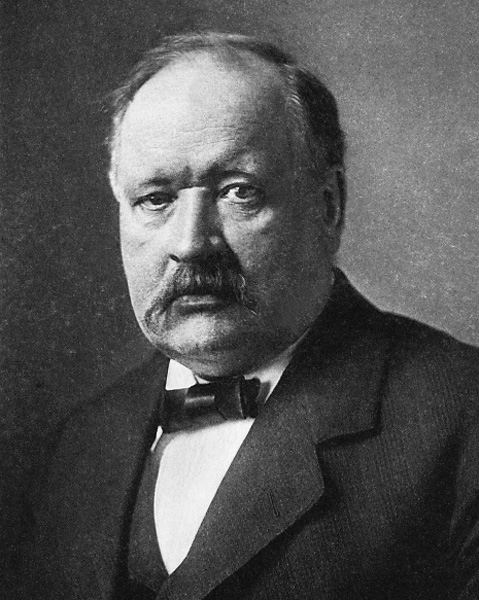
\includegraphics[width=0.22\linewidth]{images/book2/arrhenius.jpg}

{\small Svante Arrhenius (1859--1927), in 1909.}
\end{omfigure}

\section{Oefeningen}

\begin{exercise}[$\star$]\label{exo:b1:rate-laws:1}
Voor \ce{2N2O5 -> 4NO2 + O2} bij constant volume ontstaat stikstofdioxide
met $\qty{2.0e-4}{mol.L^{-1}.s^{-1}}$. Geef de \omterm{def:b1:rate-laws:rate}{reactiesnelheid}, de
\omterm{def:b1:rate-laws:rate}{vormingssnelheid} van dizuurstof en de \omterm{def:b1:rate-laws:rate}{verdwijningssnelheid} van
\ce{N2O5}.
\end{exercise}

\begin{exercise}[$\star$]\label{exo:b1:rate-laws:2}
Geef de eenheid van de \omterm{def:b1:rate-laws:order}{snelheidsconstante} voor de \omterm{def:b1:rate-laws:order}{totale ordes} 0, 1, 2
en 3, met concentraties in \unit{mol/L} en tijden in seconden.
\end{exercise}

\begin{exercise}[$\star$]\label{exo:b1:rate-laws:3}
Een eerste-ordereactie $\mathrm{A} \longrightarrow \mathrm{B}$ heeft $k = \qty{3.0e-3}{s^{-1}}$. Bereken
haar \omterm{def:b1:rate-laws:half-life}{halveringstijd} en de fractie \ce{A} die na \qty{10}{min} overblijft.
\end{exercise}

\begin{exercise}[$\star$]\label{exo:b1:rate-laws:4}
Wanneer de beginconcentratie van een beginstof gehalveerd wordt,
verdubbelt haar \omterm{def:b1:rate-laws:half-life}{halveringstijd}. Wat is de orde? En als de \omterm{def:b1:rate-laws:half-life}{halveringstijd}
gehalveerd wordt?
\end{exercise}

\begin{exercise}[$\star\star$]\label{exo:b1:rate-laws:5}
De concentratie van een beginstof \ce{A} ($\mathrm{A} \longrightarrow \mathrm{P}$) wordt gemeten: bij $t
= 0$, 10, 20, 30 en \qty{40}{min} is $[\ce{A}] = 0.100$, 0.0741, 0.0549,
0.0407 en \qty{0.0301}{mol/L}. Bepaal de orde en de \omterm{def:b1:rate-laws:order}{snelheidsconstante}.
\end{exercise}

\begin{exercise}[$\star\star$]\label{exo:b1:rate-laws:6}
Voor $\mathrm{A} + \mathrm{B} \longrightarrow \mathrm{P}$ is $v_0 = \qty{2.0e-6}{mol.L^{-1}.s^{-1}}$ voor $[\ce{A}]_0
= [\ce{B}]_0 = \qty{0.010}{mol/L}$; \qty{8.0e-6}{} als $[\ce{A}]_0$
verdubbeld wordt; \qty{4.0e-6}{} als $[\ce{B}]_0$ verdubbeld wordt.
Bepaal de \omterm{def:b1:rate-laws:order}{partiële ordes}, de \omterm{def:b1:rate-laws:order}{snelheidswet} en de \omterm{def:b1:rate-laws:order}{snelheidsconstante}.
\end{exercise}

\begin{exercise}[$\star\star$]\label{exo:b1:rate-laws:7}
De \omterm{def:b1:rate-laws:order}{snelheidswet} van $\mathrm{A} + \mathrm{B} \longrightarrow \mathrm{P}$ is $v = k[\ce{A}][\ce{B}]$. Met
$[\ce{B}]_0 = \qty{0.50}{mol/L}$ en $[\ce{A}]_0 = \qty{5.0e-3}{mol/L}$
verdwijnt \ce{A} volgens een eerste-ordekinetiek met een schijnbare
constante van \qty{0.012}{s^{-1}}. Verklaar en bereken $k$.
\end{exercise}

\begin{exercise}[$\star\star$]\label{exo:b1:rate-laws:8}
Een \omterm{def:b1:rate-laws:order}{snelheidsconstante} is \qty{1.0e-3}{s^{-1}} bij \qty{300}{K} en
\qty{5.0e-3}{s^{-1}} bij \qty{320}{K}. Bereken de \omterm{def:b1:rate-laws:activation-energy}{activeringsenergie} en
de \omterm{def:b1:rate-laws:order}{snelheidsconstante} bij \qty{310}{K}.
\end{exercise}

\begin{exercise}[$\star\star$]\label{exo:b1:rate-laws:9}
De reactie $2\,\mathrm{A} \longrightarrow \mathrm{P}$ heeft de \omterm{def:b1:rate-laws:order}{snelheidswet} $v = -\frac12\frac{\dd[\ce{A}]}
{\dd t} = k[\ce{A}]^2$ met $k = \qty{0.50}{L.mol^{-1}.s^{-1}}$. Bereken,
uitgaande van $[\ce{A}]_0 = \qty{0.020}{mol/L}$, de \omterm{def:b1:rate-laws:half-life}{halveringstijd} en de
concentratie na \qty{100}{s}.
\end{exercise}

\begin{exercise}[$\star\star\star$]\label{exo:b1:rate-laws:10}
Toon voor een eerste-ordereactie aan dat de tijd die nodig is om een
fractie $f$ van de beginstof te verbruiken $t_f = -\ln(1 - f)/(ak)$ is.
Vergelijk de tijden voor 50\,\%, 75\,\%, 90\,\% en 99.9\,\%, uitgedrukt
in \omterm{def:b1:rate-laws:half-life}{halveringstijden}.
\end{exercise}

\begin{exercise}[$\star\star\star$]\label{exo:b1:rate-laws:11}
Een huidpleister geeft een geneesmiddel af met een constante snelheid van
\qty{0.40}{mg/h} zolang zijn reservoir, aanvankelijk \qty{10}{mg}, niet
leeg is. Schrijf de wet van de resterende hoeveelheid op, geef de orde,
de \omterm{def:b1:rate-laws:half-life}{halveringstijd} en de tijd waarna de pleister uitgeput is. Waarom past
een kinetiek van orde nul bij een geneesmiddelenpleister?
\end{exercise}

\begin{exercise}[$\star\star\star$]\label{exo:b1:rate-laws:12}
Toon aan dat de regel ``tien graden meer, twee keer zo snel'' tussen
\qty{298.15}{K} en \qty{308.15}{K} overeenkomt met $E_a \approx
\qty{53}{kJ/mol}$. Welke factor geeft dezelfde \omterm{def:b1:rate-laws:activation-energy}{activeringsenergie} tussen
\qty{0}{\celsius} en \qty{10}{\celsius}?
\end{exercise}

\section{Probleem: de houdbaarheid van een geneesmiddel}

\begin{problem}[{Weekendprobleem --- een versnelde stabiliteitstest:
eerste-ordeafbraak bij 60\,\textdegree C, drie temperaturen, de
arrheniusgrafiek, en de houdbaarheid bij kamertemperatuur}]
\label{pb:b1:rate-laws:1}
Om de houdbaarheid $t_{90}$ van een tablet te voorspellen (de tijd waarna
10\,\% van het werkzame bestanddeel afgebroken is), bewaart een
laboratorium monsters bij hoge temperatuur en meet het het percentage
bestanddeel dat overblijft. Bij \qty{60}{\celsius}:
\begin{center}
\begin{tabular}{lccccc}
\hline
tijd (dagen) & 0 & 10 & 20 & 30 & 40 \\
resterend bestanddeel (\%) & 100.0 & 91.4 & 83.5 & 76.3 & 69.8 \\
\hline
\end{tabular}
\end{center}
Bij 40 en \qty{50}{\celsius} zijn de gevonden \omterm{def:b1:rate-laws:order}{snelheidsconstanten}
\qty{1.27e-3}{d^{-1}} en \qty{3.48e-3}{d^{-1}}. Neem $R =
\qty{8.314}{J/(mol.K)}$ en één maand $= \qty{30.4}{d}$.

\medskip
\noindent\textbf{Deel I --- De orde bij 60\,\textdegree C.}
\begin{enumerate}
  \item Bereken het verlies over elk interval van 10 dagen. Is de
        reactie van orde 0?
  \item Bereken $\ln(\%\text{ resterend})$ op elk tijdstip. Wat besluit je?
  \item Leid de \omterm{def:b1:rate-laws:order}{snelheidsconstante} $k_{60}$ af.
  \item Bereken de \omterm{def:b1:rate-laws:half-life}{halveringstijd} bij \qty{60}{\celsius}.
  \item Welk percentage blijft over na 60 dagen bij \qty{60}{\celsius}?
  \item Bereken $t_{90}$ bij \qty{60}{\celsius}.
\end{enumerate}

\medskip
\noindent\textbf{Deel II --- Houdbaarheid en orde.}
\begin{enumerate}[resume]
  \item Toon aan dat voor een eerste-ordeafbraak $t_{90} = \ln(10/9)/k$.
  \item Druk $t_{90}$ uit als fractie van de \omterm{def:b1:rate-laws:half-life}{halveringstijd}.
  \item Waarom hangt $t_{90}$ niet af van de dosis van de tablet?
  \item Waarom meten laboratoria de afbraak bij hoge temperatuur en niet
        bij \qty{25}{\celsius}?
  \item Als de afbraak van orde 2 was in het bestanddeel, zou een tablet
        die twee keer zo sterk is dan langer of minder lang houdbaar
        zijn? Verklaar.
\end{enumerate}

\medskip
\noindent\textbf{Deel III --- De arrheniusgrafiek.}
\begin{enumerate}[resume]
  \item Zet $1/T$ en $\ln k$ voor de drie temperaturen in een tabel.
  \item Bereken de richtingscoëfficiënt van de rechte door de punten bij
        40 en \qty{60}{\celsius}.
  \item Leid de \omterm{def:b1:rate-laws:activation-energy}{activeringsenergie} af.
  \item Controleer dat het punt bij \qty{50}{\celsius} op de rechte ligt.
  \item Bereken de \omterm{def:b1:rate-laws:activation-energy}{pre-exponentiële factor} $A$.
  \item Met welke factor neemt de snelheid toe tussen 25 en
        \qty{35}{\celsius}? Vergelijk met de vuistregel.
\end{enumerate}

\medskip
\noindent\textbf{Deel IV --- Kamertemperatuur.}
\begin{enumerate}[resume]
  \item Extrapoleer de \omterm{def:b1:rate-laws:order}{snelheidsconstante} naar \qty{30}{\celsius}.
  \item Bereken $t_{90}$ bij \qty{30}{\celsius}, in maanden.
  \item Een doos wordt drie dagen vergeten in een auto bij
        \qty{60}{\celsius}. Welke fractie van het bestanddeel gaat
        verloren?
  \item Verklaar het voorschrift ``bewaren beneden \qty{25}{\celsius}''.
  \item Extrapoleer de \omterm{def:b1:rate-laws:order}{snelheidsconstante} naar \qty{25}{\celsius}.
  \item Bereken de houdbaarheid $t_{90}$ bij \qty{25}{\celsius}, in dagen
        en in maanden.
\end{enumerate}
\end{problem}
